\documentclass[11pt]{article}
\usepackage{amsmath} % Math
\usepackage{amssymb} % Math symbols
\usepackage[english]{babel} % Language
\usepackage{fancyhdr} % Header
\usepackage[a4paper, total={15cm, 20cm}]{geometry} % Dimensions of the paper and the text area
\usepackage[utf8]{inputenc} % encoding in UTF, needed for umlauts if German
\usepackage{mathtools} % Text above arrows
\usepackage{msc} % Drawing MSCs
\usepackage{multicol} % Multiple columns
\usepackage[explicit]{titlesec} % Automatic section titles
\usepackage{tikz} % Diagrams
\usetikzlibrary{arrows.meta, automata, shapes, matrix,positioning}
\usepackage{enumitem}   % Enumeration item
\usepackage{float}
\usepackage{verbatim}
\usepackage{subcaption} 


% Other packages that might be useful in the future
%\usepackage{lingmacros}
%\usepackage{tree-dvips}
%\usepackage{ulem}
%\usepackage{amsthm}
%\usepackage{amsbsy}
%\usepackage{textcomp,gensymb}
%\usepackage{graphicx}
%\usepackage{mathtools}

% Custom variant of msc environment:
% - No "msc" keyword, longer partial messages
% - Increased vertical distance between messages
% - Less distance to the frame left and right
% - Less distance between header and processes
% - Less distance between footer and frame
% - Passing all given options down to the msc environment
\newenvironment{cmsc}[1][]{\msc[msc keyword={}, self message width=1.1cm, level height=0.6cm, environment distance=1.2cm, head top distance=0.75cm, foot distance=0.5cm, #1]}{\endmsc}

% No indentation at new paragraphs
\setlength{\parindent}{0pt}

% Distance between columns
\setlength{\columnsep}{1cm}
% Vertical line between columns
\setlength{\columnseprule}{0.5pt}
\def\columnseprulecolor{\color{gray}}

% Settings
\newcommand{\sheetNr}{9}

%% Header
\fancyhf{}
\pagestyle{fancy}
\lhead{Model Checking Exercise Sheet \sheetNr}
\rhead{Aaron Grabowy: 345766\\ Timo Bergerbusch: 344408\\ Felix Linhart: 318801}
\setlength{\headheight}{40pt}

%% Automatic section titles
\titleformat{\section}{\normalfont\Large\bfseries}{}{0em}{Exercise #1}
\titleformat{\subsection}{\normalfont\large\bfseries}{}{0em}{#1)}
\titleformat{\subsubsection}{\normalfont\large\bfseries}{}{0em}{#1)}

\newcommand{\U}{\text{ U }}
\newcommand{\W}{\text{ W }}

\begin{document}
	
\section{1}
\subsubsection*{$\Phi_1$}
$Sat(\Phi_1) = \{s_1,s_2,s_3,s_4\}$, since $s_0 \notin Sat(\Phi_1) \Rightarrow TS\not\models \Phi_1$
\subsubsection*{$\Phi_2$}
$Sat(\Phi_2) = \{s_4\}$, since $s_0 \notin Sat(\Phi_2) \Rightarrow TS\not\models \Phi_2$
\subsubsection*{$\Phi_3$}
$Sat(\Phi_3) = \{s_0,s_1,s_3,s_4\}$, since $\{s_0, s_3\} \subset Sat(\Phi_3) \Rightarrow TS \models \Phi_3$
\subsubsection*{$\Phi_4$}
% SAT(-(a v b)) = s0
% SAT( \exists \lozenge -(a v b)) = s0, s1, s2, s3
% all paths could go to s4 which does not fulfil the above thing
$Sat(\Phi_4) = \emptyset$, since $s_0 \notin Sat(\Phi_4) \Rightarrow TS\not\models \Phi_4$


\section{2}

\section{3}
\subsection{a}

Using the theorem of slide 27 of lec18-2-1. If a CTL formula $\Phi$ has an equivalent LTL formula $\varphi$, it can be obtained by removing the quantifiers.

Therefore we obtain the formula $\varphi = \lozenge(a \land \bigcirc a)$. Now either they are equivalent or there ex. no LTL-formula, which is equivalent to $\Phi_1$.

Now consider the following transition system $TS$: 
\begin{figure}[H]
	\centering	
	\begin{tikzpicture}[shorten >=1pt,node distance=2cm,on grid,auto]
		\node[state, initial, initial text=, label=$\{a\}$] (s1) {$s_1$};
		\node[state, above right = of s1, label = $\{a\}$] (s2) {$s_2$};
		\node[state, below right = of s1, label = $\emptyset$] (s4) {$s_4$};
		
		\path[->] (s1) edge (s2)
		          (s1) edge (s4)
		          (s4) edge[loop right] (s4)
		          (s2) edge[bend left = 40] (s4);
	\end{tikzpicture}
\end{figure}
Then $TS \not\models \lozenge(a \land \bigcirc a)$, because there is $trace(s_1s_4^\omega) = \{a\}\emptyset^\omega$.\\
But, since $Sat(a \land \exists \bigcirc a) = \{s_1\}$ and for all paths $\pi$ it holds that $s_1 \in Reach_{TS}(\pi)$ it follows that $TS \models \forall \lozenge ( a \land \exists \bigcirc a )$.\\
Since through TS it is proven that $\Phi_1$ is not equivalent to $\varphi$ we can conclude that there is no LTL-formula that is equivalent to $\Phi$.

\subsection{b}
Suppose we have an LTL-formula $\varphi$, s.t. $\varphi \equiv \forall\lozenge\exists\bigcirc\forall\lozenge \lnot a$.\\

Consider now TS $\mathcal{T}_1$:
\begin{figure}[H]
	\centering	
	\begin{tikzpicture}[shorten >=1pt,node distance=2cm,on grid,auto]
	\node[state, initial, initial text=, label=$\{a\}$] (s1) {$s_1$};
	\node[state, right = of s1, label = $\emptyset$] (s2) {$s_2$};
	
	\path[->] (s1) edge (s2)
	(s2) edge[loop right] (s2)
	(s1) edge[loop below] (s2);
	\end{tikzpicture}
\end{figure}
Since $\mathcal{T}_1 \models \forall\lozenge\exists\bigcirc\forall\lozenge \lnot a \Rightarrow \mathcal{T}_1 \models \varphi$.\\

Also consider TS $\mathcal{T}_2$:
\begin{figure}[H]
	\centering	
	\begin{tikzpicture}[shorten >=1pt,node distance=2cm,on grid,auto]
	\node[state, initial, initial text=, label=$\{a\}$] (s1) {$s_1$};
	
	\path[->] (s1) edge[loop below] (s2);
	\end{tikzpicture}
\end{figure}
Now $Traces(\mathcal{T}_2) = \{\{a\}^\omega\} \subset Traces(\mathcal{T}_1) \subset Words(\varphi)$, but $\mathcal{T}_2 \not\models \forall\lozenge\exists\bigcirc\forall\lozenge \lnot a$. \\
\textbf{Contradiction}

\section{4}
\subsection{a}
% all quite shitty.
% I understand the idea why it holds, but can not phrase it using definitions
\subsection{$1 \Rightarrow 2$}
Let $s\models_{LTL} \square a$.\\
Then for every trace $\pi = s_1s_2s_3\dots \in Traces(s)$, $s_1 = s$, we have that every $s_i \models a$, $i \ge 0$.\\
Therefore especially every path $\pi' \in Paths(s)$ rooted in $s$, fulfills $\pi' \models \square a$ and therefore $s \models_{CTL} \forall\square a$
\subsection{$2 \Rightarrow 3$}
Let $s \models_{CTL} \square a$.\\
Then for every path $\pi \in Paths(s)$ it holds that $\pi \models \square a$. \\
So every node $s'$ within $\pi$ has to fulfill $s'\models a$\\
This especially means that every $s' \in Reach_{TS}(s)$ it holds that $s' \models a$.\\
So $\forall s' \in Reach_{TS}(s) \>.\> s' \models a$

\subsection{$3 \Rightarrow 4$}
Let $\forall s' \in Reach_{TS}(s) \>.\> s' \models a$.\\
Through the given hint, we can infer that for every $s'' \in Reach_{TS}(s')$ it also holds, that $s'' \in Reach_{TS}(s)$ and therefore $s'' \models a$.\\
Now since for all $\pi' = s's''\dots \in Paths(s')$ it holds that $s'' \models a$, by definition of slide 66(73) we can rewrite it as $s' \models_{CTL} \forall\square a$.\\
And therefore infer $\forall s' \in Reach_{TS}(s) \>.\> s' \models_{CTL} \forall\square a$.

\subsection{$4 \Rightarrow 1$}
% worst explanation ever made
Let $\forall s' \in Reach_{TS}(s) \>.\> s' \models_{CTL} \forall\square a$.\\
For every possible state $s'$ it holds that $s'\models_{CTL} \forall \square a$. Taking definition on slide 66(73) into account, also every descendant state $s''$ of $s'$ has to fulfill $s'' \models a$.
Since $s \in Reach_{TS}(s)$ this means every state of every path has to model $a$, this concludes to $s \models_{LTL} \square a$

\subsection{b}
We use the theorem of slide 27 of lec18-2-1. If a CTL formula $\Phi$ has an equivalent LTL formula $\varphi$, it can be obtained by removing the quantifiers. Since the exercise is to prove the equivalence we can assume that an equivalent LTL formula exists.

$$\forall \big( a \U (b \land \forall\square a)\big) \rightsquigarrow a \U (b \land \square a)$$

$(\star)$: Now we can see that the Until-formula holds if we have consecutive $a$'s until we encounter a $b$ and have $\square a = \text{always }a$. So we have to always have $a$'s. In order to fulfill any side. This can be stated separately by using simply $\square a$. Then the formula can be simplified as follows:

\begin{align*}
&a \U (b \land \square a) & \text{with: }(\star) \\
&\equiv \square a \land (a \U (b \land \square a)) & \\
&\equiv \square a \land (true \U b) & \text{def. of }\lozenge\\
&\equiv \square a \land \lozenge b \\
\end{align*}

\section{5}
\subsection{a}
\begin{align*}
	\Phi_1 &= \forall \bigcirc ( \exists ( \lnot a \U (b \land \lnot c)) \lor \exists \square \forall \bigcirc a) & & \text{with: } \exists\square \Phi = \lnot \forall\lnot \Phi \\
	&\Leftrightarrow \forall \bigcirc ( \exists ( \lnot a \U (b \land \lnot c)) \lor \lnot \forall \lozenge \lnot \forall \bigcirc a) & & \text{with: } \forall\lozenge\Phi = \forall(true \U \Phi)\\
	&\Leftrightarrow \forall \bigcirc ( \exists ( \lnot a \U (b \land \lnot c)) \lor \lnot \forall (true \U \lnot \forall \bigcirc a)) & & \text{rewrite: } \lnot\forall\\
	&\Leftrightarrow \forall \bigcirc ( \exists ( \lnot a \U (b \land \lnot c)) \lor \exists(\forall \bigcirc a \W (\lnot true \land \forall \bigcirc a))) & & \text{rewrite } \lnot true\\
	&\Leftrightarrow \forall \bigcirc ( \exists ( \lnot a \U (b \land \lnot c)) \lor \exists(\forall \bigcirc a \W (false \land \forall \bigcirc a))) & & \text{rewrite: } false \land \Phi' = false\\
	&\Leftrightarrow \forall \bigcirc ( \exists ( \lnot a \U (b \land \lnot c)) \lor \exists(\forall \bigcirc a \W false)) \\
\end{align*}

\subsection{b}
\begin{align*}
\Phi_1 &= \forall \bigcirc ( \exists ( \lnot a \U (b \land \lnot c)) \lor \exists \square \forall \bigcirc a) & & \text{with: } \forall\bigcirc\Phi =  \lnot\exists\bigcirc\lnot\Phi\\
&\Leftrightarrow  \lnot \exists \bigcirc \lnot ( \exists ( \lnot a \U (b \land \lnot c)) \lor \exists \square \forall \bigcirc a) & & \text{with: } \forall\bigcirc\Phi =  \lnot\exists\bigcirc\lnot\Phi\\
&\Leftrightarrow \lnot \exists \bigcirc \lnot ( \exists ( \lnot a \U (b \land \lnot c)) \lor \exists \square \lnot \exists\bigcirc \lnot a)\\
&\Leftrightarrow \lnot \exists \bigcirc  ( \lnot \exists ( \lnot a \U (b \land \lnot c)) \land \lnot\exists \square \lnot \exists\bigcirc \lnot a)
\end{align*}

\subsection{c}
Let $(\star)$ be : $\forall(\Phi \W \Psi) = \lnot \exists ((\Phi \land \lnot \Psi) \U (\lnot \Phi \land \lnot \Psi)$
%and $(\star')$ be the equation: $\forall(\Psi_1 \U \Psi_2) = \lnot \exists( \lnot \Psi_2 \U (\lnot \Psi_1 \land \lnot \Psi_2)) \land \lnot \exists\square \lnot \Psi_2$
\begin{align*}
	\Phi_2 &= \forall ( \lnot a \W (b \rightarrow \forall \bigcirc c)) & & \text{with: } (star) \\	
	&\Leftrightarrow \lnot \exists ((\lnot a \land \lnot (b \rightarrow \forall \bigcirc c)) \U (\lnot \lnot a \land \lnot (b \rightarrow \forall \bigcirc c)) & & \text{simplify and de Morgan} \\
	&\Leftrightarrow \lnot \exists ((\lnot a \land \lnot (\lnot b \lor \forall \bigcirc c)) \U (a \land \lnot (\lnot b \lor \forall \bigcirc c)) & & \text{simplify}\\
	&\Leftrightarrow \lnot \exists ((\lnot a \land b \land \lnot\forall \bigcirc c) \U (a \land b \land \lnot \forall \bigcirc c)) & & \text{with: } \lnot \forall \bigcirc \Phi = \exists \bigcirc \lnot \Phi\\
	&\Leftrightarrow \lnot \exists ((\lnot a \land b \land \exists \bigcirc \lnot c) \U (a \land b \land \exists \bigcirc \lnot c)) & & \\
\end{align*}
	
\end{document}


